\documentclass[a4paper, 12pt]{article}
\usepackage{temp}
\usepackage{epsfig,graphicx,subfigure,amsthm,amsmath, float, xcolor, changepage, mathtools, textcomp, hyperref, bm, amssymb, tcolorbox, tikz, setspace}
\usepackage{array}
\usepackage[shortlabels]{enumitem}
\usepackage[bottom]{footmisc}
\usepackage{xepersian}
\settextfont[Scale=1]{XBZar}
%\setdigitfont{XBZar}
\setlatintextfont[Scale=0.9]{Times New Roman}
\hypersetup{
	colorlinks=true,
	urlcolor=blue!70!black
}

\newcolumntype{?}{!{\vrule width 1pt}}

\doublespacing
\begin{document}
\handout
{هوش مصنوعی}
{نیم‌سال اول ۰۱\lr{-}۰۰}
{دکتر محمدحسین رهبان}
{دانشکده مهندسی کامپیوتر}
{مینی پروژه اول - تئوری}
{محمدجواد هزاره}
{98101074}
\noindent
\\[-6em]
\section*{سوال ۱}
\begin{enumerate}[آ)]
	\item\begin{enumerate}[.i]
		\item
		هر حالت را می‌توان دوتایی $(i,j)$ در نظر گرفت که $i$ شماره سطری است که حشره در آن حضور دارد و $j$ شماره ستون حشره. هم‌چنین می‌دانیم 
		$i \in \{1, 2, \cdots, M\}$
		و
		$j \in \{1,2,\cdots, N\}$
		هستند.
		\item
		با توجه به دامنه‌ی مربوط به $i$ و $j$، اندازه فضای حالت برابر $MN$ خواهد بود.
	\end{enumerate}
	\item\begin{enumerate}[.i]
		\item
		هر حالت را می‌توان با دوتایی $(p_1, p_2)$ نشان داد که $p_1$ مختصات حشره اول (خود یک دوتایی به شکل $(i,j)$ است.) و $p_2$ نیز مختصات حشره دوم است.
		\item
		اگر مجموعه‌ی خانه‌های خالی نقشه را با $E$ نشان دهیم، آن‌گاه داریم
		$p_1, p_2 \in E$.
		بنابراین اندازه فضای حالت برابر
		$|E|^2$
		خواهد بود.
	\end{enumerate}
\end{enumerate}
\section*{سوال ۲}
\begin{enumerate}[آ)]
	\item
	مشخصا هر ژن در تناظر با یک شهر خواهد بود، بنابراین اگر هر کروموزوم 10 ژن داشته باشد، نگاشتی یک به یک از دورهای هامیلتونی به کروموزوم‌ها خواهیم داشت.
	\item \RTLfootnote{برگرفته از مقاله
	\href{http://www.ceng.metu.edu.tr/~ucoluk/research/publications/tspnew.pdf}{\lr{"Genetic Algorithm Solution of the TSP Avoiding Special Crossover and Mutation"}}
	}
	برای تابع \lr{crossover} به این صورت عمل می‌کنیم که نخست همانند \lr{crossover} کلاسیک، نقطه‌ای برای انجام \lr{crossover} روی کروموزم در نظر می‌گیریم. حال بر خلاف \lr{crossover} کلاسیک که از این نقطه به بعدِ کروموزم‌های والد را جابجا می‌کند، برای تولید فرزندان جدید، یک بار از این نقطه به قبل ژن‌های والد $p_1$ را به والد $p_2$ می‌دهیم و یک بار برعکس. در ادامه در رسیدن ژن‌های یک والد به والد دیگر، اگر ژنِ جایگزین‌شده در والدِ دریافت کننده‌ی ژنْ تکراری باشد، ژن قبلی‌ای که در این مکان بوده است را با ژن تکراری در والد دریافت‌ کننده جابجا می‌کنیم.
	
	به عنوان مثال والد $134256$ و $526134$ را در نظر بگیرید. می‌خواهیم از نقطه‌ی 3ام به بعد، \lr{crossover} را اعمال کنیم. برای تولید فرزند اول داریم:
	\begin{figure}[H]
		\centering
		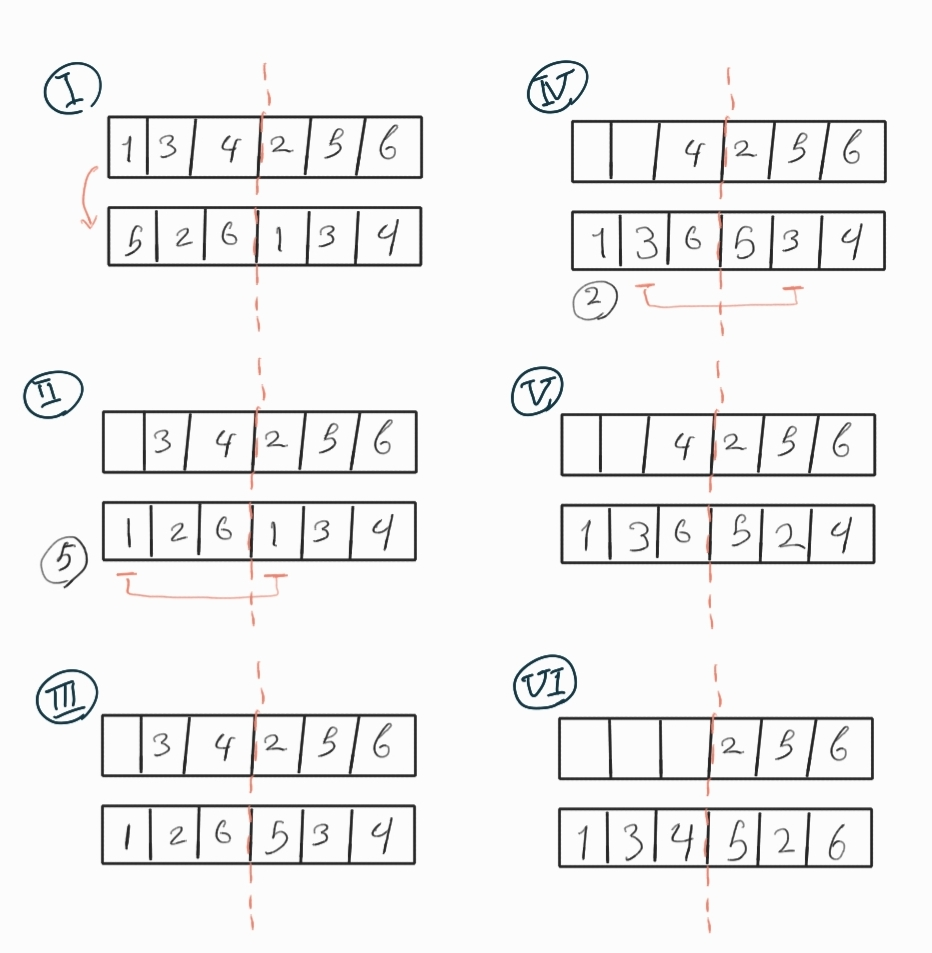
\includegraphics[width=0.7\textwidth]{crossover.jpg}
		\caption{مراحل \lr{crossover} برای تولید یکی از فرزندان}
	\end{figure}
	به طور مشابه با دادن ژن‌های والد دوم به والد اول و طی مراحل مشابه می‌توان فرزند دوم را تولید کرد.
	\item
	برای جهش می‌توان به این صورت عمل کرد که ابتدا به صورت تصادفی یکی از ژن‌ها را انتخاب کرده، و با احتمال $p$ آن را جهش می‌دهیم. برای جهش دادن نیز ژنی تصادفی و متفاوت با ژن انتخاب شده تولید کرده و به جای ژن اولیه قرار می‌دهیم. حال چون ژن جایگزین شده تکراری خواهد بود، ژن اولیه را به جای ژن تکراری قرار می‌دهیم. مثلا اگر کروموزم $546231$ را در نظر بگیریم و فرض کنیم احتمال جهش آن از $p$ بیش‌تر است، داریم:
	\[
	\begin{aligned}
		&\quad 5462\underline{3}1 \\
		\longrightarrow &\quad 5\underline{4}6241 \\
		\longrightarrow &\quad 536241
	\end{aligned}
	\]
\end{enumerate}
\section*{سوال ۳}
\begin{enumerate}[آ)]
	\item
	با توجه به تعریف تابع \lr{fitness}:
	\[
	\begin{dcases}
		f(x_1) = 16, \quad f(x_2) = 7 \\
		f(x_3) = 26, \quad f(x_4) = 2
	\end{dcases}
	\]
	\item
	برای دو فیت‌ترین کروموزم‌ها:
	\[
	\begin{dcases}
		x_1 = 765384 \\
		x_3 = 928313
	\end{dcases}
	\quad\implies\quad
	\begin{dcases}
		\widetilde{x_1} = 765313\\
		\widetilde{x_3} = 928384
	\end{dcases} 
	\]
	و برای دو غیر فیت‌ترین کروموزم‌ها:
	\[
	\begin{dcases}
		x_2 = 903642 \\
		x_4 = 232384
	\end{dcases}
	\quad\implies\quad
	\begin{dcases}
		\widetilde{x_2} = 902384 \\
		\widetilde{x_4} = 233684
	\end{dcases}
	\]
	\item
	برای کروموزم‌های حاصل داریم:
	\[
	\begin{dcases}
		f(\widetilde{x_1}) = 22, \quad f(\widetilde{x_2}) = 6 \\
		f(\widetilde{x_3}) = 20, \quad f(\widetilde{x_4}) = 1 \\
	\end{dcases}
	\]
	\item
	مشخصا با توجه به تابع \lr{fitness} ارائه شده، کروموزم بهینه برابر با $999009$ خواهد بود.
	\item
	خیر - با استفاده از \lr{crossover} فقط جای اعداد تغییر می‌کند و فرکانس یا فراوانی ژن‌ها تغییری نمی‌کند. از آن‌جایی که فراوانی عدد ۹ در کروموزم بهینه ۴ است، و فراوانی این ژن در جمعیت ابتدایی ۲ است، امکان ندارد فقط با اعمال \lr{crossover} داده شده به کروموزم بهینه دست پیدا کنیم.
\end{enumerate}
	
\end{document}



